\subsection*{3.4\quad 深度学习基础}
\subsubsection*{3.4.1\quad 深度学习与表示学习}

\noindent \textbf{一\quad 深度学习的真正定位}

\noindent 在开始学习深度学习之前,先要澄清一个常见的误解。很多人把深度学习、监督学习、强化学习当作同一层级的概念来理解,仿佛它们是几种不同的学习方法。这种理解是不准确的。

\noindent 更准确的说法是,前面3.3节讨论的监督学习、无监督学习、强化学习描述的是训练信号从哪里来、学习目标如何定义。而深度学习描述的是用什么样的函数族来表示规律、用什么方式来训练这个函数族。用更通俗的话说,监督学习告诉你这道题有标准答案,无监督学习让你自己从数据中找规律,强化学习教你通过尝试与错误学会做决策。至于用什么样的工具来完成这些任务,可以用简单的线性模型,也可以用复杂的深度网络。

\noindent 同一套深度网络,既可以在监督信号下训练,比如给定图片识别是什么物体;也可以在无监督或自监督目标下训练,比如从大量文本中学习语言规律;还可以作为强化学习中策略与价值函数的逼近器,用于下围棋或控制机器人。把这一点讲清楚,读者就不会把深度学习与监督学习或强化学习误认为同一层级的概念。

\noindent \textbf{二\quad 多层复合与分层表示}

\noindent 从最抽象的角度看,深度学习使用的是多层可微函数的复合。什么意思呢,就是把很多简单的变换一层一层串联起来,每一层都对上一层的结果再做一次变换,最终得到想要的输出。

\noindent 具体来说,给定输入$x$,一个$L$层的前向计算可以写成
\[h^{(0)}=x,\qquad h^{(\ell)}=f_\ell\!\left(h^{(\ell-1)};\theta_\ell\right)\ \ (\ell=1,\dots,L),\qquad \hat y=h^{(L)}.\]
其中$h^{(\ell)}$是第$\ell$层的中间表示,$\theta_\ell$是该层参数,整体参数记为$\theta=\{\theta_\ell\}_{\ell=1}^L$。把这些层串起来,就得到一个整体函数
\[ \hat y=f(x;\theta)=f_L\!\left(\cdots f_2(f_1(x;\theta_1);\theta_2)\cdots;\theta_L\right).\]

\noindent 这组表达式的意义非常直接。深度网络并不是某一种特定结构,而是一种分层表示的计算框架。每一层把上一层的表示变换成新的表示,早期层通常更贴近原始输入形式,后期层逐步变得更抽象、更贴近任务目标。

\medskip
\noindent \textbf{【此处添加深度网络分层示意图,展示输入层、隐藏层、输出层的层次结构与信息流动】}

\noindent 以图像识别为例。假设输入是一张照片,第一层可能识别出简单的边缘和纹理,第二层把边缘组合成形状或纹理模式,第三层把形状组合成局部物体部件,最后一层识别出完整的物体。这个过程就像我们在看一幅画,先看到线条和色块,再看出形状,最后理解画面表达的意思。深度网络所做的就是把这个认知过程用数学方式表达出来。

\noindent \textbf{三\quad 表示学习与端到端训练}

\noindent 深度学习与表示学习的关系在于,它不仅学习最后一层的判别边界或输出规则,也同时学习中间层的特征表示。传统做法常把特征工程作为独立环节。先人为设计特征,再用相对简单的模型去拟合。举个例子,要识别农作物是否患病,传统方法是先手工设计特征,比如叶片的颜色分布、病斑的大小数量等,然后用逻辑回归或支持向量机分类。深度学习把这两件事合并成一个整体。特征提取与任务学习由同一个目标函数驱动,并通过同一次训练过程共同完成。

\noindent 换句话说,深度学习的关键不在于层数多,而在于用端到端的方式让模型自己形成有用的中间表示。模型不再需要人工告诉它应该关注哪些特征,而是从大量数据中自己学习哪些特征对任务有用。

\medskip
\noindent \textbf{【此处添加端到端训练与传统两阶段流程对比示意图,左侧为传统"特征工程+模型拟合"两步走,右侧为深度学习端到端训练】}

\noindent \textbf{四\quad 训练目标的数学形式}

\noindent 深度学习通常被写成一个优化问题。以最常见的监督学习为例,给定数据集$\mathcal D=\{(x_i,y_i)\}_{i=1}^n$,选择损失函数$L(\cdot,\cdot)$来衡量预测$\hat y_i=f(x_i;\theta)$与真实$y_i$的偏差,训练目标是最小化平均损失,并常加入正则项控制复杂度:
\[ \min_{\theta}\; J(\theta)=\frac{1}{n}\sum_{i=1}^n L\big(y_i,f(x_i;\theta)\big)+\lambda\,\Omega(\theta).\]

\noindent 这一形式与前面3.3节的监督学习完全一致,差别仅在于此处的$f(x;\theta)$是由多层复合构成的高容量函数族。正因为容量高,深度网络能够拟合更复杂的输入与输出关系,但也更依赖合理的训练策略与泛化控制,否则容易出现训练不稳定或过拟合。

\noindent \textbf{五\quad 为何需要深度}

\noindent 深度之所以重要,可以从两个角度理解。第一,函数复合带来更强的表达能力。许多复杂映射若用单层或浅层模型表达,需要非常多的参数,而用多层结构往往可以用更少的参数通过逐层组合来实现。就像搭积木,用大量散乱的积木可以拼出任何形状,但如果用预先组合好的模块来搭建,效率会高得多。

\noindent 第二,分层表示更贴合许多现实数据的生成结构。以视觉为例,低层模式如边缘与纹理可以组合成局部形状,局部形状再组合成更高层语义。以语言为例,局部词组关系可以组合成句法结构,再组合成更抽象的语义关系。深度网络的层次结构相当于提供了一种逐层抽象的建模方式,使模型更容易以可复用的组件来组织复杂规律。

\noindent \textbf{六\quad 训练如何实现}

\noindent 不过表达能力强并不自动意味着训练就容易。深度网络训练依赖梯度法,通过反向传播高效计算$\nabla_\theta J(\theta)$,再用梯度下降或其变体更新参数
\[ \theta\leftarrow \theta-\eta \nabla_\theta J(\theta),\]
其中$\eta$是学习率。

\noindent 对读者而言,此处需要抓住一个核心事实。深度学习并没有绕开传统学习理论的基本约束,它只是把可表示的函数空间扩展得更大,并通过可微分计算图与梯度优化使大规模参数学习成为可能。后续所有训练技巧,比如初始化、归一化、正则化、优化器、数据增强,都可以理解为在这个高容量、强非线性的函数空间里,让梯度优化更稳定,让学到的表示更可泛化。

\noindent \textbf{七\quad 小结}

\noindent 这一节的结论是,深度学习可以被理解为用多层可微函数进行表示学习,并用端到端的梯度优化在数据上拟合参数。它与监督学习、无监督学习、强化学习的关系,是模型与训练机制对学习范式的支撑关系。理解这一点后,读者就能在后续章节自然地接受卷积神经网络、Transformer等具体结构。它们是在同一深度学习框架下,为不同数据形态引入不同的结构偏好与计算方式。
\subsubsection*{3.4.2\quad 前向计算与训练机制}

\noindent \textbf{一\quad 训练闭环的核心思想}

\noindent 深度学习最需要把握的,不是某一种网络结构的细节,而是一套稳定的计算与训练闭环。网络如何把输入变成输出,训练又如何把输出与目标之间的差距反过来变成参数更新。只要这条闭环清晰,后面无论遇到卷积神经网络还是Transformer,都可以把它们看作是在同一训练机制下更换了不同的前向计算模块。

\noindent 这套闭环包含四个环节。前向计算把输入变成输出,损失函数把输出与真实标签的差距量化成一个数,反向传播把这个差距分解到每个参数上,优化器根据梯度信息更新参数。四个环节循环往复,直到模型性能不再提升或达到预定训练轮数。

\noindent \textbf{二\quad 前向计算:逐层重编码}

\noindent 神经网络的前向计算可以概括为线性变换与非线性变换的交替复合。具体来说,设输入为$x\in\mathbb R^{d_0}$,第$\ell$层的线性部分为
\[ z^{(\ell)} = W^{(\ell)}h^{(\ell-1)} + b^{(\ell)},\qquad h^{(0)}=x,\]
其中$W^{(\ell)}\in\mathbb R^{d_\ell\times d_{\ell-1}}$是权重矩阵,$b^{(\ell)}\in\mathbb R^{d_\ell}$是偏置向量,$h^{(\ell-1)}$是上一层输出。随后通过激活函数得到
\[ h^{(\ell)}=\phi\!\left(z^{(\ell)}\right).\]
把这些层按顺序串起来,就得到一个复合函数$f(x;\theta)$,其中参数$\theta=\{W^{(\ell)},b^{(\ell)}\}_{\ell=1}^L$。

\noindent 直观上,这相当于把输入逐层重编码。前几层往往形成更局部、更简单的模式,中间层把这些模式组合成更抽象的表示,最后一层把抽象表示映射为任务需要的输出。以识别农作物病害为例,第一层可能识别叶片的颜色和纹理,第二层识别病斑的形状,第三层识别病斑的分布模式,最后一层输出是什么病害以及严重程度。

\medskip
\noindent \textbf{【此处添加神经网络前向计算示意图,展示从输入层到输出层的逐层变换过程,每层标注线性变换和激活函数】}

\noindent \textbf{三\quad 为何需要非线性激活}

\noindent 非线性在这里是不可缺少的。如果把所有激活函数$\phi$都去掉,那么多层线性变换的复合仍然等价于一次线性变换,网络再深也只能表达线性关系。激活函数提供了弯折空间,使得网络能够表示复杂的非线性决策边界或非线性函数。

\noindent 举个简单的例子。假设真实数据分布是弯弯曲曲的,如果只能用直线去拟合,无论怎么调整都很难贴合得好。但如果可以用很多段折线组合起来,就能很好地逼近这条曲线。激活函数的作用就是让每一层都可以产生一次"弯折",多层叠加就能表达足够复杂的形状。

\noindent 常见的激活函数包括ReLU、tanh、sigmoid等。但在理解训练机制的层面,重要的不是它们的具体形状,而是它们让网络从线性模型跃迁为非线性模型。ReLU是最常用的选择,它的形式非常简单,即把负数变成零而保持正数不变,但实际效果却很好,而且计算效率高。

\noindent \textbf{四\quad 输出层如何与任务对齐}

\noindent 前向计算的最后一步需要与任务类型对齐。回归问题往往直接输出实数向量$\hat y$。二分类问题通常输出一个概率$\hat p\in(0,1)$。多分类问题输出每个类别的概率分布。对应地,输出层常见写法为
\[ \hat y = g\!\left(W^{(L)}h^{(L-1)}+b^{(L)}\right),\]
其中$g$取决于任务。

\noindent 二分类时常用sigmoid函数:
\[ \hat p=\sigma(z)=\frac{1}{1+e^{-z}},\]
它把任何实数映射到$0$到$1$之间,可以解释为正类的概率。

\noindent 多分类时常用softmax函数:
\[ \hat p_k=\frac{e^{z_k}}{\sum_{j=1}^K e^{z_j}},\]
它把$K$个实数转换成一个概率分布,所有输出都非负且和为$1$。$K$就是类别总数。

\noindent 把输出解释为概率的意义在于,训练目标可以自然地写成让真实标签在模型输出分布下尽可能大,从而得到标准的对数似然与交叉熵形式。这使得训练过程有明确的统计解释。

\noindent \textbf{五\quad 损失函数定目标}

\noindent 训练机制从损失函数开始。给定样本$(x_i,y_i)$,网络前向得到预测$\hat y_i=f(x_i;\theta)$,损失函数$L(y_i,\hat y_i)$衡量预测与真实的差异。训练的目标是最小化训练集上的平均损失,必要时加正则化:
\[ J(\theta)=\frac{1}{n}\sum_{i=1}^n L\big(y_i,f(x_i;\theta)\big)+\lambda\Omega(\theta),\quad \theta^\ast=\arg\min_\theta J(\theta).\]

\noindent 这一步把学得好不好变成了一个明确的数值优化问题。监督学习与深度学习在这里并没有本质差异,差异只在于$f(\cdot;\theta)$的形式更复杂、参数更多、表达能力更强。

\noindent \textbf{六\quad 反向传播传什么}

\noindent 真正让深度学习变得可训练的是反向传播与基于梯度的优化。反向传播并不是另一套独立的学习规则,它只是把链式法则系统化地应用到计算图上,用高效的方式计算出$\nabla_\theta J(\theta)$。训练的一步更新可以写成
\[ \theta \leftarrow \theta-\eta \nabla_\theta J(\theta),\]
其中$\eta$是学习率。

\noindent 直观地理解,前向计算告诉我们现在网络输出什么、错在哪里。反向传播告诉我们这些错误分别应该归因到哪些参数上、每个参数该往哪个方向改才能让损失下降。梯度就是这种该怎么改的定量化信号。

\noindent 为了把反向传播在传什么说清楚,可以用误差信号的传播来描述。对第$\ell$层,定义该层线性输出$z^{(\ell)}$上的误差信号
\[ \delta^{(\ell)}=\frac{\partial J}{\partial z^{(\ell)}}.\]
那么参数梯度可以写成
\[ \frac{\partial J}{\partial W^{(\ell)}}=\delta^{(\ell)}(h^{(\ell-1)})^\top,\qquad \frac{\partial J}{\partial b^{(\ell)}}=\delta^{(\ell)}.\]
而误差信号在层与层之间的传播满足
\[ \delta^{(\ell)}=\big((W^{(\ell+1)})^\top \delta^{(\ell+1)}\big)\odot \phi'\!\left(z^{(\ell)}\right),\]
其中$\odot$表示按元素相乘。

\medskip
\noindent \textbf{【此处添加反向传播误差信号回传示意图,展示误差如何从输出层逐层回传到输入层】}

\noindent 这个式子表达的含义很朴素。上一层的误差来自下一层误差的回传,再乘上本层激活函数在当前位置的导数,表示本层输出的微小变化会对整体损失产生多大的影响。反向传播之所以高效,是因为它把整网的梯度计算拆成了局部的矩阵运算,并且把中间量缓存下来复用,避免了重复计算。

\noindent \textbf{七\quad 如何实现高效训练}

\noindent 实践中很少用全量梯度下降,而是用小批量随机梯度下降。把数据按批次划分,每次用一个批次近似整体梯度:
\[ \nabla_\theta J(\theta)\approx \frac{1}{|B|}\sum_{i\in B}\nabla_\theta L\big(y_i,f(x_i;\theta)\big),\]
然后更新参数。

\noindent 这样做一方面计算更高效,每次不需要遍历全部数据就能做一次参数更新。另一方面这种带噪声的梯度反而在一定程度上有助于跳出不佳的局部区域,让训练更容易找到更好的解。优化器可以是基础的随机梯度下降,也可以加入动量或自适应学习率如Adam。但在机制层面,它们都在做同一件事,用梯度信息决定参数更新方向,并用不同的方式调节更新幅度与稳定性。

\noindent \textbf{八\quad 小结}

\noindent 这一节最终需要读者形成的稳固认识是,深度学习的训练并不依赖某种神秘技巧,它是一套明确的计算流程。前向把输入变成输出,损失把输出与目标的差距量化,反向把差距分解为对各层参数的责任,优化器据此更新参数。网络结构改变的是前向计算的形式与归纳偏置,但训练闭环保持不变。理解这一点,读者才能在后续学习卷积神经网络的卷积算子或Transformer的注意力算子时,把注意力放在新算子如何改变表示与信息流动,而不是重新学习一套完全不同的训练逻辑。
\subsubsection*{3.4.3\quad 卷积神经网络基础}

\noindent \textbf{一\quad 卷积神经网络的核心思想}

\noindent 卷积神经网络之所以适合处理图像,并不因为它采用了与其他神经网络完全不同的训练机制。它同样遵循前向计算、损失函数、反向传播、梯度更新的训练闭环。卷积神经网络的关键变化发生在前向计算的结构设计上。它把图像数据中最常见、最稳定的规律写进网络结构,使网络在学习时天然倾向于提取边缘、角点、纹理等局部模式,并保持这些模式在空间上的分布信息。

\begin{figure}[htbp]
\centering
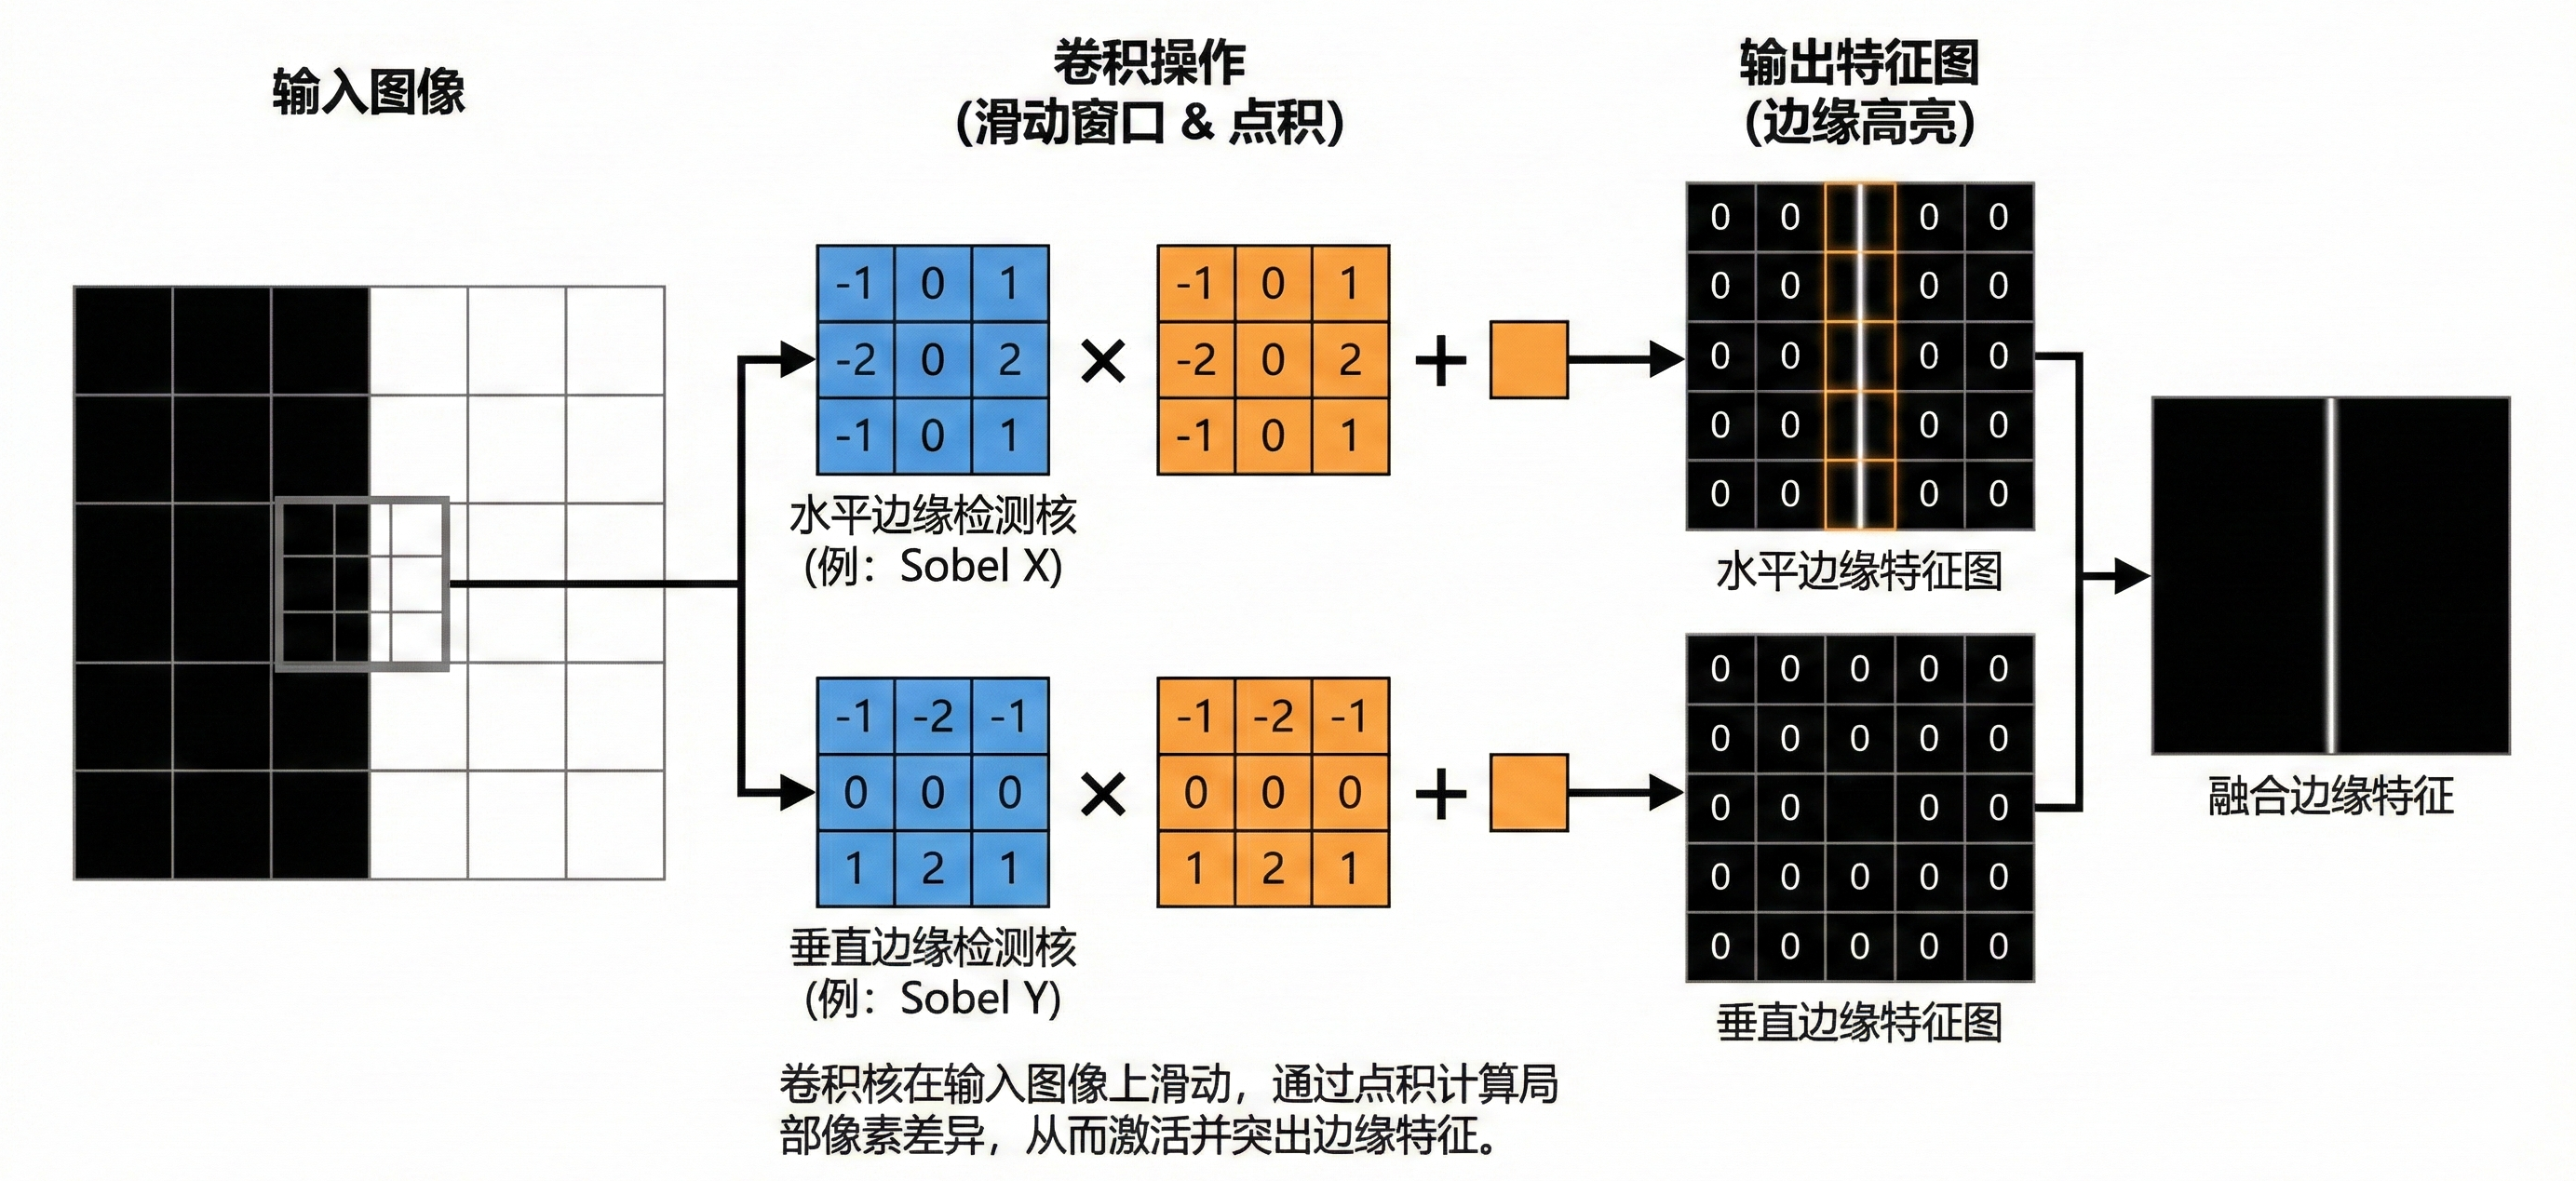
\includegraphics[width=0.9\textwidth]{figures/fig-cnn-sliding-window}
\caption{卷积核在输入图像上滑动,对边界产生响应。左侧是输入图像,中间展示卷积核以滑动窗口方式在局部区域计算,右侧输出特征图在边界位置形成一条亮带,表示该位置附近与卷积核所偏好的模式高度匹配。}
\label{fig:cnn-sliding-window}
\end{figure}

\noindent 图\ref{fig:cnn-sliding-window}给出了一个典型示意。左侧输入图像中存在一条明显的垂直边界,中间展示卷积核以滑动窗口方式在局部区域计算,右侧输出特征图在边界位置形成一条亮带。这条亮带就是边界响应,表示该位置附近与卷积核所偏好的模式高度匹配。

\noindent \textbf{二\quad 卷积层的基本计算}

\noindent 在最常见的二维情形中,输入是一张二维网格(例如灰度图像)$X\in\mathbb R^{H\times W}$。卷积层用一个小的权重矩阵(卷积核)$W\in\mathbb R^{k\times k}$在输入上滑动。图中标注的滑动窗口展示的就是这种滑动方式。卷积核每次只覆盖输入图像的一块局部区域,并在该局部窗口上做加权求和,得到输出特征图$Y\in\mathbb R^{(H-k+1)\times(W-k+1)}$:
\[ Y_{i,j}=\sum_{u=0}^{k-1}\sum_{v=0}^{k-1}W_{u,v}\,X_{i+u,\,j+v}+b,\]
其中$b$是偏置项。随后通常还会接一个非线性激活函数$\phi(\cdot)$得到
\[ H_{i,j}=\phi(Y_{i,j}).\]

\noindent 若输入是多通道(例如RGB图像),则$X\in\mathbb R^{H\times W\times C}$。此时卷积核可以理解为在空间维度仍是$k\times k$,但同时覆盖$C$个通道。输出每个位置的值来自对所有通道对应局部窗口的加权汇总。多个卷积核会产生多个输出通道,从而形成更丰富的特征表示。就本节的目的而言,理解单通道卷积的核心计算已足够。

\noindent 卷积计算的直观意义,可以直接借助图中的垂直边缘探测器来理解。图中展示的卷积核数值形如
\[ \begin{pmatrix} 1&0&-1\\ 1&0&-1\\ 1&0&-1 \end{pmatrix},\]
它可以看作一个垂直边缘探测器。对窗口左侧像素做正向加权,对窗口右侧像素做负向加权。若滑动窗口落在一块灰度相对均匀的区域,左右差异不大,加减后输出接近$0$。若滑动窗口跨过黑白分界,左右差异显著,加减后输出幅度变大。于是右侧输出特征图在边界位置出现亮带,这就是卷积核对垂直边缘这一局部模式的强响应。

\noindent 需要强调的是,这类核在示意图中是人为构造用于解释的。在真实卷积神经网络中,卷积核的数值由训练自动学得,但训练得到的早期卷积核常常会呈现与边缘、方向、纹理相关的响应特性,这与图示直觉是一致的。

\noindent \textbf{三\quad 局部连接:为什么只看一小块}

\noindent 卷积层的每一个输出单元只连接输入的一小块区域,这一小块区域称为感受野。对前式而言,$Y_{i,j}$只依赖$X$的一个$k\times k$子矩阵。图中蓝色的局部窗口就是感受野的可视化。卷积核无论移动到哪里,都只在这一小块区域内进行计算,而不会直接把整张图像的所有像素一次性混合。

\noindent 局部连接来自对图像数据的基本判断。图像的关键结构往往由局部像素组合决定。边缘是局部灰度突变,纹理是局部重复模式,角点是局部方向变化。与其让网络在第一层就把整张图像的所有像素彼此相连,不如先在局部范围内学习可复用的小特征,再逐层把小特征拼成更大的结构。图中右侧那条亮带的出现,本质上就是在每个位置对这一小块区域是否存在垂直边缘给出的局部判别结果。

\noindent 局部连接直接带来两个结果。第一,参数数量显著下降。若用全连接层把$H\times W$个像素直接映射到$m$个隐藏单元,参数量是$mHW$量级。而卷积层对单个卷积核只需要$k^2$个参数(多通道时是$k^2C$),与图像的空间尺寸无关。第二,学习更稳定。模型更少依赖远距离像素之间偶然的相关性,而更集中于局部可重复的规律,这通常会改善训练的样本效率并降低过拟合风险。

\noindent \textbf{四\quad 权重共享:为什么同一个卷积核要到处用}

\noindent 卷积层最具识别性的设计,是同一个卷积核$W$在所有空间位置重复使用。图中权重共享强调:无论滑动窗口位于输入图像的哪个位置,使用的都是同一组权重。也就是说,卷积层并不是每个位置都学一个探测器,而是学一个探测器在所有位置通用。

\noindent 这背后的直觉是,某种局部模式(例如垂直边缘)可能出现在图像的任何位置,而检测这种模式的方法不应随位置改变。权重共享因此有两层价值。其一是压缩参数规模,使模型容量不会随着输入尺寸的增加而失控。其二是提升泛化能力与样本效率。模型一旦学到一个有效的局部模式探测器,就能在整张图上复用,而不需要在每个位置分别见到大量样本才能学会同一种模式。

\noindent \textbf{五\quad 平移等变:输入平移会带来怎样的输出变化}

\noindent 卷积的另一个关键性质是平移等变。图中右侧的输出特征图给出了最直观的呈现。输入图像中的边界在哪里,输出特征图中的亮带就出现在对应位置。如果把输入边界整体向左或向右移动,输出中的亮带也会随之移动。换言之,卷积层既能告诉你有没有这种模式,也能保留模式出现在哪里。

\noindent 用算子语言表达,如果$T_\Delta$表示把输入平移$\Delta$的操作,$\mathrm{Conv}$表示卷积操作,那么在忽略边界效应的理想条件下,有近似关系:
\[ \mathrm{Conv}(T_\Delta X)=T_\Delta(\mathrm{Conv}(X)).\]
这就是平移等变:输入发生平移,输出以同样方式平移,响应形态保持一致。

\noindent 平移等变与平移不变需要区分。卷积层本身保留位置信息,因此输出会跟随输入一起移动,这是等变。而许多分类任务希望最终判别结果对目标位置不敏感(不变),这通常需要进一步的结构或训练策略来弱化位置依赖,例如池化、步幅下采样、全局平均池化,或通过数据增强让模型在不同位置都见过目标。常见的整体策略是:前几层保留空间细节以便检测局部结构,后几层逐步扩大感受野并降低分辨率,使表示更位置鲁棒,最终得到更接近平移不变的判别特征。

\noindent \textbf{六\quad 一个可手算的卷积计算实例}

\noindent 图中用一个$3\times3$的垂直边缘检测核来说明卷积核在整幅图上扫描会在边界处产生强响应。下面给出一个更小的手算例子,目的不是复现图中的具体亮带,而是让读者把滑动窗口的加权求和落到可计算的步骤上。

\noindent 考虑一个$3\times3$的输入矩阵
\[ X=\begin{pmatrix} 1&2&0\\ 0&1&3\\ 2&1&1 \end{pmatrix},\]
取一个$2\times2$卷积核
\[ W=\begin{pmatrix} 1&0\\ 0&-1 \end{pmatrix},\quad b=0.\]
采用步幅$1$、无填充,则输出$Y$为$2\times2$。逐位置计算如下。

\noindent 左上角位置$(i=0,j=0)$对应窗口$\begin{pmatrix}1&2\\0&1\end{pmatrix}$,因此
\[ Y_{0,0}=1\cdot 1+0\cdot 2+0\cdot 0+(-1)\cdot 1=0.\]

\noindent 右上角位置$(0,1)$对应窗口$\begin{pmatrix}2&0\\1&3\end{pmatrix}$,因此
\[ Y_{0,1}=1\cdot 2+0\cdot 0+0\cdot 1+(-1)\cdot 3=-1.\]

\noindent 左下角位置$(1,0)$对应窗口$\begin{pmatrix}0&1\\2&1\end{pmatrix}$,因此
\[ Y_{1,0}=1\cdot 0+0\cdot 1+0\cdot 2+(-1)\cdot 1=-1.\]

\noindent 右下角位置$(1,1)$对应窗口$\begin{pmatrix}1&3\\1&1\end{pmatrix}$,因此
\[ Y_{1,1}=1\cdot 1+0\cdot 3+0\cdot 1+(-1)\cdot 1=0.\]

\noindent 汇总可得
\[ Y=\begin{pmatrix} 0&-1\\ -1&0 \end{pmatrix}.\]
如果再接一个ReLU激活$\phi(t)=\max(0,t)$,则
\[ H=\begin{pmatrix} 0&0\\ 0&0 \end{pmatrix}.\]
这表示:对这个输入而言,该卷积核在各个位置都没有产生正向响应。换一个卷积核,或者换一幅输入图像,输出就可能在某些位置变大,形成清晰的局部响应图。图中的边界亮带就是这种现象在特定卷积核与特定输入上的典型结果。卷积核对某类模式敏感,于是当滑动窗口扫过该模式出现的位置时,输出特征图在对应位置显著变亮。

\noindent \textbf{七\quad 小结}

\noindent 本节需要读者牢固掌握的是,卷积层仍然是线性变换的一种,但它通过局部连接与权重共享把参数组织成可在全图复用的局部探测器,从而带来平移等变这一关键性质。理解这一点,后续再学习多通道卷积、步幅与填充、池化、残差结构等内容,就会更容易把握它们各自改变了什么、又保留了什么。
\subsubsection*{3.4.4\quad Transformer 基础}

\medskip
\begin{figure}[htbp]
\centering
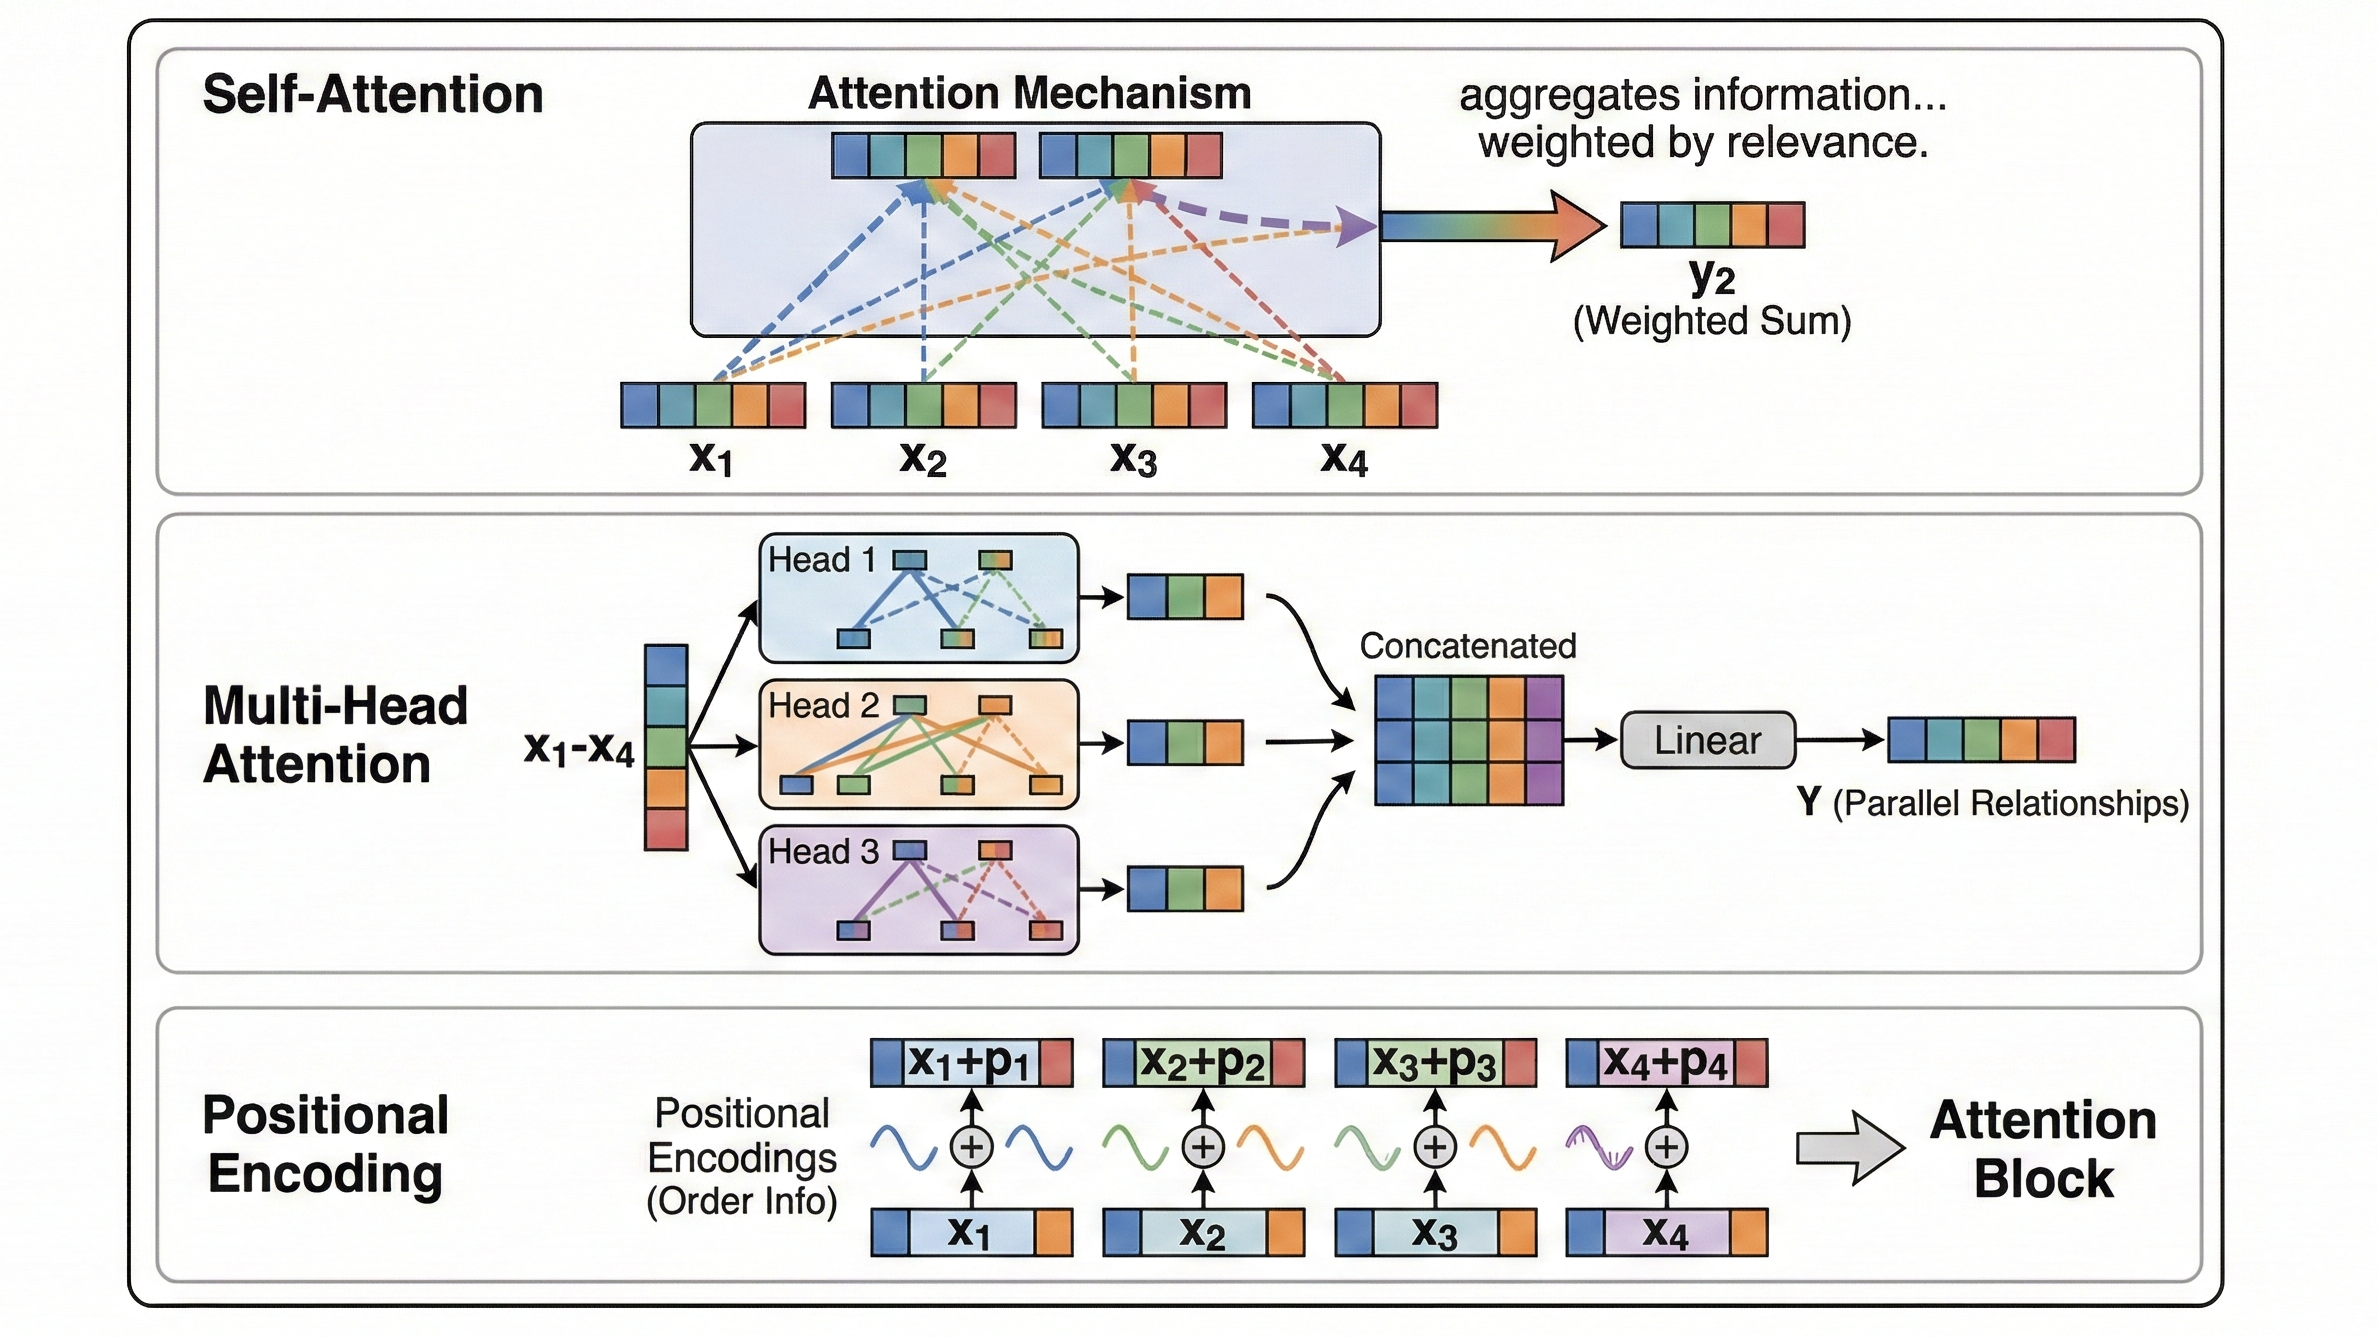
\includegraphics[width=0.9\textwidth]{figures/fig-transformer-attention}
\caption{Transformer 的三个核心机制:自注意力、多头注意力和位置编码。}
\label{fig:transformer-attention}
\end{figure}

\medskip
\noindent 图~\ref{fig:transformer-attention}~展示了 Transformer 结构的三个核心机制。左侧部分是自注意力,它让序列中每个位置都能看到其他所有位置的信息,并根据相关性进行加权汇总。中间部分是多头注意力,它并行地使用多组注意力来捕捉不同类型的关系。右侧部分是位置编码,它把位置信息注入到输入表示中。理解这三部分,就掌握了 Transformer 的基础。

\medskip
\noindent \textbf{一\quad 自注意力:序列位置间的直接交互}

\medskip
\noindent 图\ref{fig:transformer-attention}中左侧的自注意力部分展示了 Transformer 与传统网络最本质的区别。在循环网络中,信息需要沿着时间步一步一步传递,前面的信息要等到后面才能用上。在卷积网络中,信息主要在局部邻域内传播,想看到很远的位置需要堆叠很多层。而 Transformer 通过自注意力机制,让序列中任意两个位置都可以在一次计算中直接交互。

\medskip
\noindent 具体来说,设输入序列长度为 $n$,每个位置的表示维度为 $d$。把输入表示堆叠成矩阵 $X\in\mathbb R^{n\times d}$,其中第 $i$ 行 $x_i^\top$ 表示第 $i$ 个 token 的向量表示。这里的 token 可以是词、子词、帧或 patch 等基本单元。

\medskip
\noindent 自注意力的核心思想是对序列中每个位置 $i$,模型会根据内容相关性在所有位置 $j$ 上分配权重,然后把这些位置的表示按权重加权求和。你可以把它想象成每个位置都在问,序列中哪些位置对我最重要,我应该向它们借信息。

\medskip
\noindent 在计算上 Transformer 先把同一个输入 $X$ 线性映射成三组向量,即查询、键、值:
\[ Q=XW_Q,\qquad K=XW_K,\qquad V=XW_V, \]
其中 $W_Q,W_K,W_V\in\mathbb R^{d\times d_k}$,因此 $Q,K,V\in\mathbb R^{n\times d_k}$。

\medskip
\noindent $q_i$ 可以理解为位置 $i$ 想找什么信息的表达,$k_j$ 是位置 $j$ 提供什么信息的标签,$v_j$ 则是位置 $j$ 真正要被汇聚的内容。图\ref{fig:transformer-attention}中左侧的连接线就是在展示这种查询与键的匹配过程,线越粗表示相关性越强。

\medskip
\noindent 接着计算注意力权重矩阵。对任意两个位置 $i,j$,它们的相关性由点积 $q_i^\top k_j$ 给出,并做缩放与 softmax 归一化:
\[ A=\mathrm{softmax}\!\left(\frac{QK^\top}{\sqrt{d_k}}\right),\qquad A\in\mathbb R^{n\times n}. \]
其中 $A_{i,j}$ 表示在更新位置 $i$ 的表示时对位置 $j$ 的关注程度。最后用权重对 $V$ 做加权汇总:
\[ \mathrm{Attn}(X)=AV,\qquad \mathrm{Attn}(X)\in\mathbb R^{n\times d_k}. \]

\medskip
\noindent 图\ref{fig:transformer-attention}中左侧展示的正是这个过程。每个位置都向其他所有位置发出查询,根据点积得到相关性分数,softmax 把这些分数变成归一化的权重,最后用这些权重对所有位置的值进行加权求和。这样每个位置的新表示就包含了整个序列的信息,而信息量的大小由相关性决定。

\medskip
\noindent \textbf{二\quad 多头注意力:从多个角度捕捉关系}

\medskip
\noindent 图\ref{fig:transformer-attention}中中间部分展示了多头注意力的结构。单头注意力在同一个相似度空间里衡量相关,但序列中的相关性往往不止一种。以语言为例,有的词之间语义相近,有的词之间存在语法依赖,有的词在句法结构上紧密相关,还有的词共同构成了某个主题。如果只用一种相似度度量,很难同时捕捉所有这些关系。

\medskip
\noindent 多头注意力用并行的多组线性映射来表达多种相关性视角。设有 $h$ 个头,第 $t$ 个头计算
\[ \mathrm{head}_t=\mathrm{Attn}(XW_Q^{(t)},XW_K^{(t)},XW_V^{(t)}), \]
然后把各头输出拼接并再做一次线性变换:
\[ \mathrm{MHA}(X)=\mathrm{Concat}(\mathrm{head}_1,\dots,\mathrm{head}_h)\,W_O. \]

\medskip
\noindent 图\ref{fig:transformer-attention}中中间的多个并行方块就是在展示这种结构。每个头有自己独立的 $W_Q,W_K,W_V$,因此每个头在不同的表示空间里计算注意力。有的头可能更关注语法关系,有的头可能更关注语义相似,有的头可能更关注长距离依赖。多头注意力让模型能同时从多个角度在全序列范围内查找并汇聚信息,而不是把所有关系压缩到一种相似度度量里。

\medskip
\noindent \textbf{三\quad 位置编码:注入顺序信息}

\medskip
\noindent 图\ref{fig:transformer-attention}中右侧部分展示了位置编码的必要性。注意力机制本身只依赖向量间的点积相似度,它并不关心 token 出现在第几个位置。如果你把输入序列的顺序打乱,注意力计算的结果也会相应打乱,但计算形式本身并不会因为顺序变化而自动感知。

\medskip
\noindent 这对语言、时间序列等任务是个问题。词序变了,意思往往就变了。时间戳的位置不同,事件的意义也不同。因此 Transformer 需要显式地把位置信息注入到输入表示中。

\medskip
\noindent 最常见的做法是位置编码。设 $P\in\mathbb R^{n\times d}$ 为位置向量矩阵,将其与输入相加:
\[ X' = X + P. \]
这样模型在计算 $Q,K,V$ 时就同时看到了内容信息和位置信息。位置编码可以是固定的函数形式,例如正弦余弦,也可以是可学习参数。图\ref{fig:transformer-attention}中右侧展示的就是把位置信息叠加到输入表示上的过程。

\medskip
\noindent \textbf{四\quad Transformer 的完整层结构}

\medskip
\noindent 前面介绍的三个核心机制需要组织成一个可训练的层。Transformer 的常用基本块由两部分组成,即自注意力子层与前馈网络子层。前馈网络对每个位置独立地做两层线性变换与非线性:
\[ \mathrm{FFN}(x)=W_2\,\phi(W_1x+b_1)+b_2, \]
它的作用是对每个位置的表示进行非线性变换与维度扩展或压缩,增强表达能力。自注意力负责在不同位置之间交换信息,前馈网络负责在每个位置内部做更强的非线性加工。两者交替堆叠,就形成了 Transformer 的深层表示学习。

\medskip
\noindent 在深层网络中稳定训练往往依赖残差连接与归一化。常见写法是:
\[ H_1 = \mathrm{LN}(X + \mathrm{MHA}(X)), \]
\[ H_2 = \mathrm{LN}(H_1 + \mathrm{FFN}(H_1)). \]

\medskip
\noindent 残差连接使信息与梯度能够更顺畅地在深层网络中流动,归一化则缓解数值尺度的漂移,使优化更稳定。你可以把它理解为,注意力与前馈模块负责做变换,残差与归一化负责让变换可堆叠、可训练。

\medskip
\noindent \textbf{五\quad 一个可手算的注意力示例}

\medskip
\noindent 为了把自注意力从公式落到可计算的步骤上,下面用一个极简数值示例展示相关性、权重、加权汇总的过程。考虑三个 token 的表示,为便于手算维度取 $2$,并直接给出某一头的 $Q,K,V$:
\[ q_1=(1,0),\quad q_2=(0,1),\quad q_3=(1,1), \]
\[ k_1=(1,0),\quad k_2=(0,1),\quad k_3=(1,1), \]
\[ v_1=(1,0),\quad v_2=(0,1),\quad v_3=(1,1). \]

\medskip
\noindent 以位置 $3$ 为例,它对三个位置的未归一化相关性即点积为
\[ q_3^\top k_1=1,\quad q_3^\top k_2=1,\quad q_3^\top k_3=2. \]
这些分数通过 softmax 变成权重。在这个简单例子中,位置 $3$ 对自身的相关性最大,因此会最关注位置 $3$ 本身,同时也会一定程度关注位置 $1$ 与位置 $2$。最终输出是
\[ o_3=\sum_{j=1}^3 a_{3j} v_j, \]
也就是把三处的信息按权重加权融合。这个例子表达的要点是,注意力不是选一个位置,而是对多个位置分配权重并融合,因此它能够在一次计算中把全局依赖直接写入每个位置的表示。

\medskip
\noindent \textbf{六\quad 小结}

\medskip
\noindent Transformer 的基础可以归结为图~\ref{fig:transformer-attention}~展示的三个核心机制。自注意力通过 $QK^\top$ 建立位置间的相关性,用 softmax 把相关性变成可解释的权重,再用权重对 $V$ 做加权汇总,从而让序列中任意位置在一次计算中直接交互。多头注意力让这种交互具有多种并行视角,位置编码补上顺序信息,残差连接与归一化使深层堆叠可训练。理解这些机制后,读者再去学习更具体的 Transformer 变体,例如编码器或解码器结构、掩码注意力、交叉注意力、长序列改进等时,会更清楚每一处改动究竟是在改变信息如何流动,以及改变了哪些计算代价与归纳偏置。
